%
% Appendix 2
%

\chapter{Boosted Decision Trees}
\label{app:bdts}
Boosted Decision Trees are the single MVA/machine learning technique used for discriminating signal from background
in this analysis. BDTs are a special instance of a decision tree, which is illustrated below in Figure~\ref{fig:dec_tree}.
This analysis uses the BDT implementation in the Toolkit for Multivariate Analysis (TMVA) software~\cite{tmva}.
The choice of BDTs over other MVA methods such as artificial neural networks (aNNs) or support vector machines (SVMs) is motivated
by several factors. 

\begin{figure}[hbtp]
 \begin{center}
   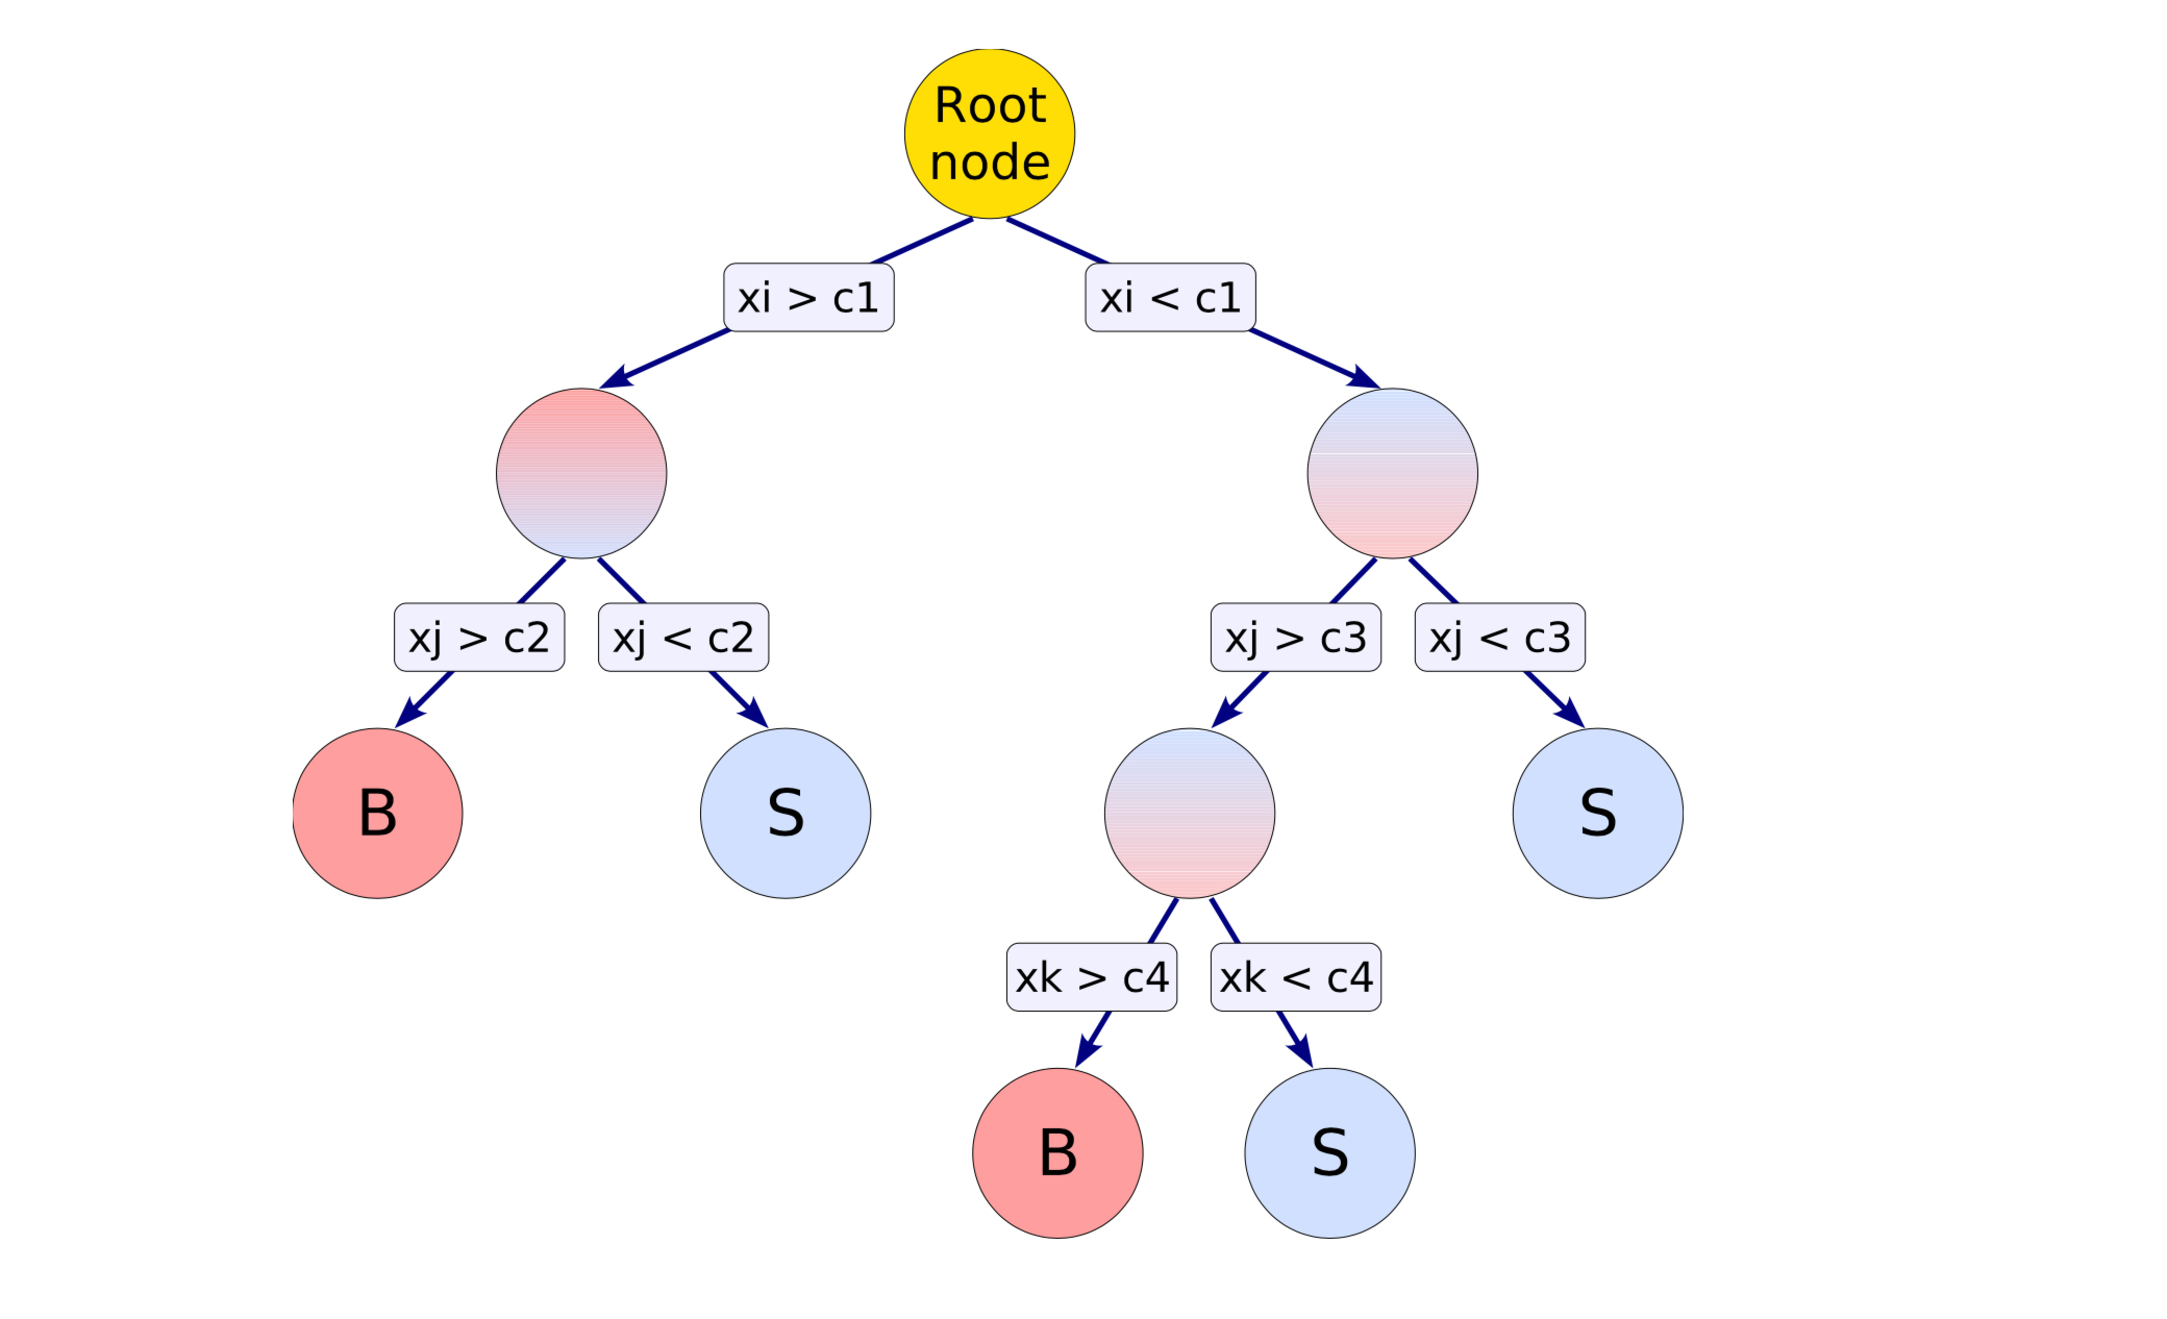
\includegraphics[width=0.8\textwidth]{ap2_figs/decision_tree.pdf}
   \caption[A decision tree diagram.]{An overview diagram of a single decision tree. The decision nodes are a mixture of red and blue,
     while the terminal nodes or leaves, are ideally depicted colored red or blue and labeled S or B for signal or background respectively~\cite{tmva}.}
   \label{fig:dec_tree}
 \end{center}
\end{figure}

\section{Tree Growth}

\section{Boosting}


